% Provenance (never printed): see sources/outline_sources.md (Year 2: radiogenic tracers
% Sr, Nd, Pb and mantle reservoirs; crustal growth; stable isotopes, delta notation and
% fractionation, d18O and d13C). Curves from figdata/bachelor-2/isotopes.py; exercise and
% problem values in the Book 4 scratch calculators calc/ch04.py and calc/ch04pb.py.
% Ruling (Sync 2): delta value and fractionation factor are chemistry's (Year 3 volume),
% recalled; this chapter defines the reference standards and the meteoric water line.
\chapter{समस्थानिक भू-रसायन}\label{ch:b2:isotope-geochemistry}

दक्षिणी प्रशांत में मंगाइया और दक्षिणी अटलांटिक में ट्रिस्टन दा कुन्हा,
दोनों बेसाल्ट से बने ज्वालामुखीय द्वीप हैं, और एक का हस्त-नमूना
दूसरे के हस्त-नमूने जैसा, या किसी मध्य-महासागरीय कटक के नमूने जैसा ही दिखता है।
उनके समस्थानिक उन्हें अलग बताते हैं। मंगाइया के बेसाल्टों के स्ट्रॉन्शियम में
स्ट्रॉन्शियम-87 का वही अनुपात है जो कटकों में है, लगभग
$^{87}\mathrm{Sr}/^{86}\mathrm{Sr} = 0.7028$, जबकि उनका सीसा पृथ्वी पर सबसे
रेडियोजनित सीसों में है, कटकों के 18.4 के सामने $^{206}\mathrm{Pb}/^{204}\mathrm{Pb}$
लगभग 21.6। ट्रिस्टन के बेसाल्टों में अधिक स्ट्रॉन्शियम-87 है, 0.7050 से
0.7054, और दोनों से कम नियोडिमियम-143। गलन इन भारी तत्त्वों के समस्थानिकों को
नहीं छाँटता, इसलिए हर लावा उस प्रावार का समस्थानिक चिह्न लिए होता है
जो उसे बनाने के लिए पिघला: पृथ्वी का प्रावार एक भंडार नहीं बल्कि
कई भंडार है, जिन्होंने अरबों वर्षों तक भिन्न जनक--संतति अनुपात बनाए
रखे हैं। यह अध्याय रुबिडियम, सैमेरियम, यूरेनियम
और थोरियम के रेडियोधर्मी क्षय को अनुरेखकों के एक समुच्चय के रूप में प्रयोग करता है, नियोडिमियम समस्थानिकों के माध्यम से प्रावार और
महाद्वीपीय भूपर्पटी के विकास का अनुसरण करता है, प्रावार को
भंडारों और भंडारों के मिश्रणों में बाँटता है, चर्चा करता है कि महाद्वीप कितनी तेज़ी से बढ़े,
और ऑक्सीजन, हाइड्रोजन और कार्बन के हल्के स्थायी समस्थानिकों के साथ समाप्त होता है, जो
पृथ्वी में जल और कार्बन का अनुरेखण करते हैं।
% ledger: data:b4-oib-isotopes, gale13:isotopes

\begin{recall}
कोई रेडियोधर्मी जनक $\lambda P$ की दर से क्षय होता है, और बंद तंत्र में
संतति-अनुपात $(D/D_s)_{\text{अब}} = (D/D_s)_0 + (P/D_s)_{\text{अब}}
(e^{\lambda t}-1)$ के अनुसार बढ़ता है, जहाँ $D_s$ संतति का एक स्थायी समस्थानिक है; साथ बने खनिज या
चट्टानें एक समकालरेखा पर स्थित होती हैं, जिसकी प्रवणता आयु देती है और जिसका
अंतःखंड आरंभिक अनुपात देता है (पुस्तक 2, कक्षा 12; पुस्तक 3,
रेडियोमितीय आयु-निर्धारण का अध्याय)। द्रव्यमान स्पेक्ट्रोमीटर आयनों को उनके
द्रव्यमान-आवेश अनुपात से पृथक करता है (रसायन-विज्ञान की पुस्तकें, द्वितीय वर्ष)। किसी नमूने का $\delta$ मान
$\delta = (R_{\text{नमूना}}/R_{\text{मानक}} - 1)\times 1000$ है, प्रति
मिल में, और दो प्रावस्थाओं A और B के बीच प्रभाजन गुणांक
$\alpha_{\mathrm{A/B}} = R_{\mathrm A}/R_{\mathrm B}$ है, जहाँ $R$
भारी और हल्के समस्थानिक का अनुपात है; दोनों, समस्थानिक प्रभाजन उत्पन्न करने वाली शून्य-बिंदु ऊर्जाओं के
साथ, रसायन-विज्ञान की पुस्तकों के तृतीय वर्ष में प्रस्तुत किए गए हैं।
\omterm{def:b2:elements-in-the-earth:partition}{असंगत तत्त्व}, MORB और OIB
\cref{ch:b2:elements-in-the-earth} में परिभाषित किए गए थे।
\end{recall}

\section{अनुरेखक के रूप में रेडियोजनित समस्थानिक}

तीन क्षय-तंत्र प्रावार और भूपर्पटी के बारे में अधिकांश सूचना लिए हुए हैं।
रुबिडियम-87 स्ट्रॉन्शियम-87 में क्षय होता है, सैमेरियम-147 नियोडिमियम-143 में, और यूरेनियम
तथा थोरियम, अपनी क्षय-शृंखलाओं के माध्यम से, सीसे के तीन समस्थानिकों में। हर जनक
और संतति गलन के दौरान अपने व्यवहार में भिन्न हैं, और हर संतति का एक
स्थायी, अ-रेडियोजनित समस्थानिक है जिसके सापेक्ष उसे मापा जाता है।

\begin{table}[ht]
\centering
\begin{tabular}{lllll}
\hline
जनक & संतति & मापा गया अनुपात & क्षय-स्थिरांक (प्रति वर्ष) & अर्ध-आयु (\unit{Ga})\\
\hline
$^{87}$Rb & $^{87}$Sr & $^{87}\mathrm{Sr}/^{86}\mathrm{Sr}$ & \num{1.3972e-11} & 49.6\\
$^{147}$Sm & $^{143}$Nd & $^{143}\mathrm{Nd}/^{144}\mathrm{Nd}$ & \num{6.524e-12} & 106.25\\
$^{238}$U & $^{206}$Pb & $^{206}\mathrm{Pb}/^{204}\mathrm{Pb}$ & \num{1.55125e-10} & 4.47\\
\hline
\end{tabular}
\caption{अनुरेखकों के रूप में प्रयुक्त तीन दीर्घजीवी क्षय-तंत्र। डेटा: IUPAC--IUGS
अनुशंसाएँ (Villa और अन्य, 2020 और 2022)।}
\label{tab:b2:isotope-geochemistry:decay}
\end{table}
% ledger: villa22:rb87, villa20:sm147

\begin{definition}[रेडियोजनित समस्थानिक अनुरेखक]\label{def:b2:isotope-geochemistry:tracer}
\emph{रेडियोजनित समस्थानिक अनुरेखक}\index{रेडियोजनित समस्थानिक अनुरेखक} किसी
दीर्घजीवी रेडियोधर्मी जनक से उत्पन्न संतति समस्थानिक का उसी तत्त्व के एक स्थायी
समस्थानिक से अनुपात है, जैसे $^{87}\mathrm{Sr}/^{86}\mathrm{Sr}$ या
$^{143}\mathrm{Nd}/^{144}\mathrm{Nd}$, जिसका प्रयोग किसी चट्टान की आयु बताने के बजाय
उसके स्रोत की पहचान के लिए होता है। किसी भंडार का अनुपात उसके
जनक--संतति अनुपात द्वारा तय दर से बढ़ता है, और इसलिए उस अनुपात का इतिहास दर्ज करता है।
\end{definition}

जब भी प्रावार पिघलता है, क्षय-युग्म के दोनों तत्त्व अलग हो जाते हैं।
\cref{ch:b2:elements-in-the-earth} में रुबिडियम स्ट्रॉन्शियम से अधिक असंगत
और नियोडिमियम सैमेरियम से अधिक असंगत सिद्ध हुआ। इसलिए गलित, और उससे बनने वाली भूपर्पटी,
ऊँचे Rb/Sr और निम्न Sm/Nd के साथ प्रावार को छोड़ते हैं; अवशेष
निम्न Rb/Sr और ऊँचा Sm/Nd रखता है। समय के साथ भूपर्पटी अपने स्रोत से तेज़
स्ट्रॉन्शियम-87 और धीमे नियोडिमियम-143 प्राप्त करती है; \omterm{def:b2:isotope-geochemistry:reservoirs}{क्षीणित
प्रावार} इसका उलटा करता है। दोनों युग्मों के अनुपात विपरीत
दिशाओं में चलते हैं, यह बात नीचे का Sr--Nd आरेख स्पष्ट करता है।

\begin{proposition}[समस्थानिक अनुपात गलन में बचे रहते हैं]\label{prop:b2:isotope-geochemistry:melting}
जब कोई चट्टान पिघलती है और गलित अवशेष से अलग होता है, तो गलित के
$^{87}\mathrm{Sr}/^{86}\mathrm{Sr}$ और $^{143}\mathrm{Nd}/^{144}\mathrm{Nd}$ अनुपात
मापन की परिशुद्धता के भीतर स्रोत के अनुपातों के बराबर होते हैं;
केवल जनक--संतति अनुपात, Rb/Sr और Sm/Nd, बदलते हैं।
\end{proposition}
\admitted

\noindent यह कथन दो तथ्यों पर टिका है। किसी एक तत्त्व के समस्थानिकों की
इलेक्ट्रॉनिक संरचना समान होती है, इसलिए वे क्रिस्टल या गलित में लगभग समान रूप से प्रवेश करते हैं;
स्ट्रॉन्शियम-87 और स्ट्रॉन्शियम-86 के बीच सापेक्ष द्रव्यमान-अंतर, लगभग एक
प्रतिशत, ऑक्सीजन या हाइड्रोजन की तुलना में कहीं छोटा है, और उच्च तापमान पर
किसी साम्य प्रभाजन गुणांक का लघुगणक तापमान के वर्ग के व्युत्क्रम के अनुसार
घटता है, 1 की ओर। और स्वयं मापन द्रव्यमान स्पेक्ट्रोमीटर में होने वाले
प्रभाजन को दो अ-रेडियोजनित समस्थानिकों का एक अनुपात नियत करके संशोधित करता है
(नियोडिमियम के लिए $^{146}\mathrm{Nd}/^{144}\mathrm{Nd} =
0.7219$), जो किसी भी छोटे प्राकृतिक प्रभाजन को भी मिटा देता। इसलिए कोई लावा
अपने स्रोत के समस्थानिक अनुपातों का नमूना लेता है, जबकि उसके अनुरेखी-तत्त्व
अनुपात गलन को भी प्रतिबिंबित करते हैं।
% ledger: white:chur, white:t-dependence

\section{प्रावार और भूपर्पटी का विकास}

\subsection{कॉन्ड्राइटी भंडार}

सैमेरियम और नियोडिमियम दोनों दुर्गलनीय शिलारागी दुर्लभ मृदाएँ हैं
(\cref{ch:b2:elements-in-the-earth}): \omterm{def:b2:elements-in-the-earth:bse}{समग्र सिलिकेट पृथ्वी} को उनका
कॉन्ड्राइटी अनुपात बनाए रखना चाहिए था। तब \omterm{def:b2:planet-formation-meteorites:chondrule}{कॉन्ड्राइट}
अविभेदित पृथ्वी का Sm--Nd इतिहास देते हैं।

\begin{definition}[कॉन्ड्राइटी एकसमान भंडार]\label{def:b2:isotope-geochemistry:chur}
\emph{कॉन्ड्राइटी एकसमान भंडार}\index{कॉन्ड्राइटी एकसमान भंडार}
(CHUR) \omterm{def:b2:planet-formation-meteorites:chondrule}{कॉन्ड्राइटों} के सैमेरियम--नियोडिमियम संघटन वाला एक मॉडल भंडार है,
जो सौरमंडल के निर्माण से बंद है। इसके वर्तमान
अनुपात $(^{143}\mathrm{Nd}/^{144}\mathrm{Nd})_{\mathrm{CHUR}} = 0.512638$ और
$(^{147}\mathrm{Sm}/^{144}\mathrm{Nd})_{\mathrm{CHUR}} = 0.1966$ हैं।
\end{definition}
% ledger: white:chur

समकालरेखा समीकरण से पीछे की ओर चलाने पर, जब प्रथम ठोस
\qty{4567}{Myr} पहले संघनित हुए (\cref{ch:b2:planet-formation-meteorites}), तब CHUR का अनुपात था
\[
  ^{143}\mathrm{Nd}/^{144}\mathrm{Nd} = 0.512638 - 0.1966\,\bigl(e^{\lambda\cdot
  \num{4.567e9}\,\mathrm{yr}}-1\bigr) = 0.506692 .
\] तब से इसका अनुपात
1.2 प्रतिशत बढ़ा है। स्थलीय चट्टानों के बीच के अंतर हज़ार गुना
छोटे हैं, और अधिक सुविधाजनक इकाई में बताए जाते हैं।
% ledger: lugaro:cai, villa20:sm147

\begin{definition}[एप्सिलॉन संकेतन]\label{def:b2:isotope-geochemistry:epsilon}
\emph{एप्सिलॉन संकेतन}\index{एप्सिलॉन संकेतन} किसी नमूने के
$^{143}\mathrm{Nd}/^{144}\mathrm{Nd}$ अनुपात को, वर्तमान से पहले के समय $t$ पर,
उसी समय CHUR से उसके सापेक्ष विचलन के रूप में, प्रति दस
हज़ार भागों में व्यक्त करता है:
\[
  \varepsilon_{\mathrm{Nd}}(t) = \left(
  \frac{(^{143}\mathrm{Nd}/^{144}\mathrm{Nd})_{\text{नमूना}}(t)}
       {(^{143}\mathrm{Nd}/^{144}\mathrm{Nd})_{\mathrm{CHUR}}(t)} - 1\right)\times 10^4 .
\]
समय के बिना, $\varepsilon_{\mathrm{Nd}}$ वर्तमान मान है।
\end{definition}

माध्य MORB का, जिसका $^{143}\mathrm{Nd}/^{144}\mathrm{Nd} = 0.513074$ है,
$\varepsilon_{\mathrm{Nd}} = (0.513074/0.512638 - 1)\times10^4 = +8.5$ है; अधिकांश चट्टानें
$-20$ और $+10$ के बीच हैं। धनात्मक मान का अर्थ है कि चट्टान के स्रोत का
Sm/Nd, पृथ्वी के इतिहास में औसतन, \omterm{def:b2:planet-formation-meteorites:chondrule}{कॉन्ड्राइटों} से ऊँचा रहा है:
वह अधिक \omterm{def:b2:elements-in-the-earth:partition}{असंगत तत्त्व}, नियोडिमियम, में क्षीणित है। ऋणात्मक
मान का अर्थ इसका उलटा है। कॉन्ड्राइटी Sm/Nd से विचलन
भिन्नात्मक विचलन से मापा जाता है
\[
  f_{\mathrm{Sm/Nd}} = \frac{(\mathrm{Sm}/\mathrm{Nd})_{\text{नमूना}}}
  {(\mathrm{Sm}/\mathrm{Nd})_{\mathrm{CHUR}}} - 1,
\]
जो अनुपात द्रव्यमान से हों या परमाणुओं से, एक ही रहता है। \cref{ch:b2:elements-in-the-earth}
के CI मानों (Sm 0.145, Nd \qty{0.457}{ppm},
$\mathrm{Sm}/\mathrm{Nd} = 0.317$) के साथ, ऊपरी महाद्वीपीय भूपर्पटी (4.7 और
\qty{27}{ppm}, 0.174) का $f_{\mathrm{Sm/Nd}} = -0.45$ है।
% ledger: gale13:isotopes, white:chur, lodders:ci-table, rg03:ucc-trace

\begin{proposition}[$\varepsilon_{\mathrm{Nd}}$ की रैखिक वृद्धि]\label{prop:b2:isotope-geochemistry:linear}
जो भंडार CHUR से अलग हुआ और तब से भिन्नात्मक विचलन
$f_{\mathrm{Sm/Nd}}$ बनाए रखे है, वह अपना $\varepsilon_{\mathrm{Nd}}$, समय में
आगे की ओर, इस दर से बदलता है:
\[
  \frac{\mathrm{d}\varepsilon_{\mathrm{Nd}}}{\mathrm{d}\tau} \approx Q\,f_{\mathrm{Sm/Nd}},
  \qquad
  Q = 10^4\,\lambda_{147}\,
  \frac{(^{147}\mathrm{Sm}/^{144}\mathrm{Nd})_{\mathrm{CHUR}}}
       {(^{143}\mathrm{Nd}/^{144}\mathrm{Nd})_{\mathrm{CHUR}}}
  = \qty{25.0}{\per\giga\year},
\]
जहाँ $\tau$ आगे की ओर गिना गया समय है। जिस भंडार का अलगाव के समय मान $\varepsilon_0$ था,
एक समय $T$ पहले, उसका आज $\varepsilon_{\mathrm{Nd}} \approx \varepsilon_0
+ Q f_{\mathrm{Sm/Nd}} T$ है।
\end{proposition}

\begin{proof}
$R$ को $^{143}\mathrm{Nd}/^{144}\mathrm{Nd}$ के लिए और $p$ को
$^{147}\mathrm{Sm}/^{144}\mathrm{Nd}$ के लिए लिखिए। बंद भंडार में
$\mathrm{d}R/\mathrm{d}\tau = \lambda p\,e^{\lambda t}$, जहाँ $t$ वर्तमान से पहले का
समय है; चूँकि $\lambda t \le 0.03$, गुणक $e^{\lambda t}$ 1 से अधिकतम
3 प्रतिशत भिन्न है, और $\mathrm{d}R/\mathrm{d}\tau \approx \lambda p$। तब
$\mathrm{d}(R_s - R_c)/\mathrm{d}\tau \approx \lambda (p_s - p_c) = \lambda p_c
f_{\mathrm{Sm/Nd}}$, क्योंकि $p_s/p_c - 1 = f_{\mathrm{Sm/Nd}}$। $R_c$ से भाग देने पर,
जो पृथ्वी की आयु में केवल 1.2 प्रतिशत बदलता है,
$\mathrm{d}\varepsilon/\mathrm{d}\tau \approx 10^4\lambda p_c f/R_c$ मिलता है।
$\lambda = \qty{6.524e-12}{\per\year}$, $p_c = 0.1966$ और $R_c = 0.512638$ के साथ, $Q =
\num{2.502e-8}$ प्रति वर्ष, अर्थात् \qty{25.0}{\per\giga\year}।
\end{proof}
% ledger: villa20:sm147, white:chur

इसलिए ऊपरी भूपर्पटी के Sm/Nd ($f = -0.45$) वाली भूपर्पटी CHUR के सापेक्ष प्रति अरब वर्ष लगभग
11 एप्सिलॉन इकाइयाँ खोती है, जबकि किसी प्रावार भंडार को केवल $f = +0.07$ चाहिए ताकि वह
0 से MORB मान $+8.5$ तक \qty{4.567}{Ga} में चढ़ सके। नीचे का चित्र तीन
भंडारों के लिए सटीक समीकरणों का अनुसरण करता है: CHUR, पृथ्वी के बनने से बंद एक \omterm{def:b2:isotope-geochemistry:reservoirs}{क्षीणित प्रावार}
जिसका Sm/Nd उसे आज MORB मान तक लाता है ($^{147}\mathrm{Sm}/^{144}\mathrm{Nd} =
0.211$), और उस प्रावार से 2.7 अरब वर्ष पहले निकाली गई एक भूपर्पटी, जिसका
Sm/Nd ऊपरी भूपर्पटी जैसा है ($0.108$)। भूपर्पटी $\varepsilon_{\mathrm{Nd}} =
+3.5$ पर आरंभ हुई, जो उस समय उसके स्रोत का मान था, और अब
$-27$ पर है।

\begin{definition}[क्षीणित प्रावार, समृद्ध प्रावार]\label{def:b2:isotope-geochemistry:reservoirs}
\emph{क्षीणित प्रावार}\index{क्षीणित प्रावार} प्रावार का वह भाग है जिसने
\omterm{def:b2:elements-in-the-earth:partition}{असंगत तत्त्व} गलितों को खो दिए हैं, जिससे उसका Sm/Nd ऊँचा और उसका Rb/Sr
कॉन्ड्राइटी से निम्न है; समय के साथ उसका $\varepsilon_{\mathrm{Nd}}$ धनात्मक और
उसका $^{87}\mathrm{Sr}/^{86}\mathrm{Sr}$ निम्न हो जाता है। \emph{समृद्ध
प्रावार}\index{समृद्ध प्रावार} प्रावार का वह भाग है जिसने \omterm{def:b2:elements-in-the-earth:partition}{असंगत तत्त्व} प्राप्त किए हैं,
उदाहरण के लिए पुनर्चक्रित भूपर्पटी से या छोटे गलितों से,
ऋणात्मक $\varepsilon_{\mathrm{Nd}}$ या ऊँचे $^{87}\mathrm{Sr}/^{86}\mathrm{Sr}$ के साथ।
\end{definition}

\begin{omfigure}
\centering
\begin{tikzpicture}
\begin{axis}[omrecord, width=0.82\linewidth, height=6.4cm,
  x dir=reverse, xmin=0, xmax=4.6, ymin=-30, ymax=12,
  xlabel={वर्तमान से पहले का समय (\unit{Ga})}, ylabel={$\varepsilon_{\mathrm{Nd}}(t)$},
  tick label style={font=\scriptsize}, label style={font=\small}]
\addplot[thick, black] table[x=t_Ga, y=eps] {figdata/out/bachelor-2-isotopes-chur.dat};
\addplot[very thick, blue!70!black] table[x=t_Ga, y=eps] {figdata/out/bachelor-2-isotopes-dm.dat};
\addplot[very thick, brown!70!black] table[x=t_Ga, y=eps] {figdata/out/bachelor-2-isotopes-crust.dat};
\addplot[densely dashed, gray] coordinates {(2.7,-30) (2.7,12)};
\node[font=\scriptsize, anchor=north] at (axis cs:3.6,-0.6) {CHUR};
\node[font=\scriptsize, blue!70!black, anchor=south east] at (axis cs:0.4,8.8) {क्षीणित प्रावार, $+8.5$};
\node[font=\scriptsize, brown!70!black, anchor=north east] at (axis cs:0.3,-25.5) {भूपर्पटी, $-27$};
\node[font=\scriptsize, gray, anchor=north west, align=left] at (axis cs:2.65,-12) {\qty{2.7}{Ga} पर\\निकाली गई भूपर्पटी};
\end{axis}
\end{tikzpicture}
\par\smallskip{\small $\varepsilon_{\mathrm{Nd}}$ के रूप में नियोडिमियम समस्थानिकों का विकास:
कॉन्ड्राइटी भंडार का (परिभाषा से शून्य), \qty{4.567}{Ga} से बंद
एक \omterm{def:b2:isotope-geochemistry:reservoirs}{क्षीणित प्रावार} का, जिसका Sm/Nd उसे आज माध्य MORB तक लाता है, और उससे
\qty{2.7}{Ga} पहले ऊपरी महाद्वीपीय भूपर्पटी के Sm/Nd के साथ निकाली गई
एक भूपर्पटी का। हर रेखा लगभग सीधी है, जैसा रैखिक-वृद्धि प्रतिज्ञप्ति कहती है। डेटा:
CHUR, White का पाठ; माध्य MORB, Gale और अन्य (2013); भूपर्पटी का Sm/Nd,
Rudnick और Gao।}
\end{omfigure}
% ledger: white:chur, villa20:sm147, gale13:isotopes, rg03:ucc-trace, lodders:ci-table, lugaro:cai

\subsection{दो पूरक भंडार}

यदि महाद्वीपीय भूपर्पटी और \omterm{def:b2:isotope-geochemistry:reservoirs}{क्षीणित प्रावार} एक ही कॉन्ड्राइटी भंडार से बने
थे, तो उनके नियोडिमियम को जुड़कर कॉन्ड्राइटी मान देना चाहिए। नियोडिमियम
वाहक है: हर भंडार अपने द्वारा धारित नियोडिमियम के अनुपात में गिना जाता है।

\begin{proposition}[समस्थानिक द्रव्यमान-संतुलन]\label{prop:b2:isotope-geochemistry:mass-balance}
मान लीजिए भंडार $i$, जिनके द्रव्यमान $M_i$ और नियोडिमियम-सांद्रताएँ $C_i$ हैं,
एक जनक भंडार के विभाजन से आते हैं। तब, बहुत अच्छे सन्निकटन तक,
\[
  \sum_i M_i C_i\, \varepsilon_i = \Bigl(\sum_i M_i C_i\Bigr) \varepsilon_{\text{जनक}},
\]
दोनों पक्षों का मान एक ही समय पर निकाला जाता है, और जनक का अनुसरण ऐसे किया जाता है मानो
वह पूरा बना रहा हो।
\end{proposition}

\begin{proof}
$^{143}\mathrm{Nd}$ परमाणुओं की संख्या और $^{144}\mathrm{Nd}$ परमाणुओं की संख्या
दोनों विभाजन में संरक्षित रहती हैं, और बाद में हर भंडार में ठीक उसी तरह बढ़ती है
($^{143}\mathrm{Nd}$ के लिए) या स्थिर रहती है ($^{144}\mathrm{Nd}$ के लिए) जैसे
पूरे में। अतः $^{144}\mathrm{Nd}$ से भारित, अनुपातों $R_i$ का माध्य
जनक के अनुपात $R_p$ के बराबर है। नियोडिमियम में $^{144}\mathrm{Nd}$ का हिस्सा
भंडारों के बीच हज़ार में एक भाग से बहुत कम बदलता है, इसलिए
$M_iC_i$ से भारित करना $^{144}\mathrm{Nd}$ से भारित करने जैसा ही है। अंत में, किसी दिए गए समय पर $\varepsilon$
$R$ का रैखिक फलन है, $\varepsilon = 10^4(R/R_c - 1)$, और
रैखिक फलनों का भारित माध्य भारित माध्य का रैखिक फलन होता है।
\end{proof}

नियोडिमियम के ऊपरी-भूपर्पटी मान \qty{27}{ppm} को पूरी भूपर्पटी के लिए लेने पर,
\qty{2830}{kg/m^3} पर \qty{7.2e9}{km^3} की महाद्वीपीय भूपर्पटी, अर्थात्
\qty{2.0e22}{kg} या सिलिकेट पृथ्वी के द्रव्यमान का 0.51 प्रतिशत, सिलिकेट पृथ्वी के नियोडिमियम का
$0.0051\times27/1.25 = 11$ प्रतिशत धारण करती है (\omterm{def:b2:elements-in-the-earth:bse}{आद्य
प्रावार}, \qty{1.25}{ppm})। यदि भूपर्पटी का औसत $\varepsilon_{\mathrm{Nd}}$
$-15$ है, तो $0.11\times15 = 1.65$ इकाइयों के ऋणात्मक योगदान को
प्रावार को संतुलित करना होगा: MORB मान $+8.5$ वाले भंडार को सिलिकेट पृथ्वी के नियोडिमियम का
लगभग पाँचवाँ भाग धारण करना होगा (\cref{exo:b2:isotope-geochemistry:9})। यह उन
तर्कों में से एक है कि कटकों द्वारा प्रतिदर्शित \omterm{def:b2:isotope-geochemistry:reservoirs}{क्षीणित प्रावार} पूरा
प्रावार नहीं है।
% ledger: cogley84:continents, cm95:crust, ms95:pm-trace, rg03:ucc-trace, data:prem, earth:mass, gale13:isotopes

\section{प्रावार के भंडार}

महासागरीय बेसाल्टों के समस्थानिक अनुपात महाद्वीपीय भूपर्पटी से गुज़रे बिना प्रावार का
नमूना लेते हैं। एक-दूसरे के सापेक्ष आलेखित करने पर वे भूपर्पटी और \omterm{def:b2:isotope-geochemistry:reservoirs}{क्षीणित प्रावार} की
पूरकता और अन्य भंडारों के अस्तित्व, दोनों को
दिखाते हैं।

अधिकांश महासागरीय बेसाल्टों में स्ट्रॉन्शियम और नियोडिमियम समस्थानिक प्रतिसहसंबद्ध हैं:
ऊँचे $\varepsilon_{\mathrm{Nd}}$ वाले लावा का
$^{87}\mathrm{Sr}/^{86}\mathrm{Sr}$ निम्न होता है। इस पट्टी को प्रावार सरणी कहते हैं; यह
गलन के दौरान दोनों युग्मों के विपरीत व्यवहार से निकलती है (रुबिडियम स्ट्रॉन्शियम से कम
संगत, सैमेरियम नियोडिमियम से अधिक संगत)। माध्य
MORB इसके क्षीणित सिरे पर है, $^{87}\mathrm{Sr}/^{86}\mathrm{Sr} = 0.702819$ और
$\varepsilon_{\mathrm{Nd}} = +8.5$ के साथ। \omterm{def:b2:elements-in-the-earth:morb-oib}{महासागरीय द्वीप बेसाल्ट} वहाँ से
निम्नतर $\varepsilon_{\mathrm{Nd}}$ और उच्चतर $^{87}\mathrm{Sr}/^{86}\mathrm{Sr}$ की ओर फैलते हैं, पर
एक ही रेखा के अनुदिश नहीं।
% ledger: white:dm, gale13:isotopes

\begin{definition}[प्रावार अंत्य-सदस्य]\label{def:b2:isotope-geochemistry:end-members}
\emph{प्रावार अंत्य-सदस्य}\index{प्रावार अंत्य-सदस्य} उन चरम
समस्थानिक संघटनों में से एक है जिनके मिश्रण से महासागरीय
बेसाल्टों के Sr, Nd और Pb समस्थानिक अनुपात बनाए जा सकते हैं। सामान्यतः चार के नाम लिए जाते हैं: DMM, क्षीणित
MORB प्रावार (निम्न $^{87}\mathrm{Sr}/^{86}\mathrm{Sr}$, ऊँचा $\varepsilon_{\mathrm{Nd}}$);
HIMU, अपने स्रोत में ऊँचे $\mu = {}^{238}\mathrm{U}/^{204}\mathrm{Pb}$ के कारण
(अत्यंत रेडियोजनित सीसा, $^{206}\mathrm{Pb}/^{204}\mathrm{Pb}$ 20 से ऊपर, निम्न
$^{87}\mathrm{Sr}/^{86}\mathrm{Sr}$ के साथ); EM1, \omterm{def:b2:isotope-geochemistry:reservoirs}{समृद्ध प्रावार} 1 (मध्यम रूप से ऊँचा
$^{87}\mathrm{Sr}/^{86}\mathrm{Sr}$, ऋणात्मक $\varepsilon_{\mathrm{Nd}}$, अ-रेडियोजनित
सीसा); और EM2, \omterm{def:b2:isotope-geochemistry:reservoirs}{समृद्ध प्रावार} 2 (ऊँचा $^{87}\mathrm{Sr}/^{86}\mathrm{Sr}$)।
\end{definition}
% ledger: white:end-members

\begin{omfigure}
\centering
\begin{tikzpicture}
\begin{axis}[omrecord, width=0.82\linewidth, height=6.6cm,
  xmin=0.7020, xmax=0.7064, ymin=-6, ymax=11,
  xlabel={$^{87}\mathrm{Sr}/^{86}\mathrm{Sr}$}, ylabel={$\varepsilon_{\mathrm{Nd}}$},
  xticklabel style={/pgf/number format/fixed, /pgf/number format/precision=4},
  scaled x ticks=false, legend pos=south west, legend cell align=left,
  legend style={font=\scriptsize}, tick label style={font=\scriptsize},
  label style={font=\small}]
\addplot[only marks, mark=*, mark size=1.3pt, red!70!black] table[x=sr, y=eps] {figdata/out/bachelor-2-isotopes-himu.dat};
\addlegendentry{HIMU प्रकार: सेंट हेलेना, मंगाइया, तुबुआई}
\addplot[only marks, mark=square*, mark size=1.2pt, brown!70!black] table[x=sr, y=eps] {figdata/out/bachelor-2-isotopes-em1.dat};
\addlegendentry{EM1 प्रकार: ट्रिस्टन दा कुन्हा, गफ़}
\addplot[only marks, mark=diamond*, mark size=3pt, blue!70!black] table[x=sr, y=eps] {figdata/out/bachelor-2-isotopes-morb.dat};
\addlegendentry{माध्य MORB}
\addplot[densely dashed, gray] coordinates {(0.7020,0) (0.7064,0)};
\node[font=\scriptsize, gray, anchor=south east] at (axis cs:0.7063,0.1) {CHUR};
\draw[->, gray] (axis cs:0.7030,9.5) -- (axis cs:0.7046,0.8);
\node[font=\scriptsize, gray, anchor=west, align=left] at (axis cs:0.7036,6.5) {प्रावार सरणी:\\क्षीणित से समृद्ध};
\end{axis}
\end{tikzpicture}
\par\smallskip{\small पाँच महासागरीय द्वीपों के 89 बेसाल्टों और माध्य \omterm{def:b2:elements-in-the-earth:morb-oib}{मध्य-महासागरीय कटक
बेसाल्ट} के स्ट्रॉन्शियम और नियोडिमियम समस्थानिक। HIMU-प्रकार के द्वीप
मुख्य सरणी के नीचे आते हैं, MORB के निम्न स्ट्रॉन्शियम अनुपात के साथ पर निम्नतर
$\varepsilon_{\mathrm{Nd}}$ के साथ; EM1-प्रकार के द्वीप CHUR के समृद्ध पक्ष पर हैं।
EM2 प्रकार के समोआ के लावा $^{87}\mathrm{Sr}/^{86}\mathrm{Sr} = 0.7205$ तक पहुँचते हैं, जो इस पैमाने से
दाईं ओर बहुत दूर है। डेटा: Stracke और अन्य (2022), CC BY 4.0; Gale और
अन्य (2013); Edwards और अन्य (2019)।}
\end{omfigure}
% ledger: data:b4-oib-isotopes, gale13:isotopes, edwards19:samoa, white:chur

चित्र के द्वीप-समूह यादृच्छिक नहीं हैं। सेंट हेलेना समूह,
जिसमें ऑस्ट्रल द्वीप (उनमें मंगाइया और तुबुआई) और
असेंशन आते हैं, मुख्य सरणी के नीचे आता है और उसका सीसा सबसे अधिक रेडियोजनित है
($^{206}\mathrm{Pb}/^{204}\mathrm{Pb}$ 20 से ऊपर; मंगाइया 21.5 से 22.0 तक पहुँचता है)।
करगेलेन समूह, अर्थात् ट्रिस्टन दा कुन्हा, गफ़ और करगेलेन, मध्यम रूप से ऊँचे
$^{87}\mathrm{Sr}/^{86}\mathrm{Sr}$ और ऋणात्मक $\varepsilon_{\mathrm{Nd}}$ पर है, सदा
अ-रेडियोजनित सीसे के साथ। सोसाइटी समूह, समोआ और मार्केसस के साथ, एक
कम ढलान वाली Sr--Nd प्रवृत्ति बनाता है जो बहुत ऊँचे स्ट्रॉन्शियम अनुपातों तक पहुँचती है: समोआ के दो लावाओं
के $^{87}\mathrm{Sr}/^{86}\mathrm{Sr}$ 0.7186 और 0.7205 हैं, जो आधुनिक
समुद्री जल (0.7092) से ऊँचे हैं। सेंट हेलेना, करगेलेन और सोसाइटी समूह क्रमशः HIMU,
EM1 और EM2 प्रकार हैं।
% ledger: white:end-members, data:b4-oib-isotopes, edwards19:samoa

प्रावार के दो भागों के बीच भिन्न अनुपात को लंबे समय तक जनक--संतति अनुपात के
अंतर ने बनाए रखा होगा: $\varepsilon_{\mathrm{Nd}}$ की
10 इकाइयों का अंतर, रैखिक-वृद्धि प्रतिज्ञप्ति के अनुसार, $f = 0.4$ पर 1 अरब वर्ष
या $f = 0.1$ पर 4 अरब वर्ष लेता है। इसलिए
प्रावार के भंडार पुराने हैं। वे क्या हैं, यह उन जनक--संतति अनुपातों से पढ़ा जाता है
जिनकी माँग उनके समस्थानिक करते हैं। HIMU को लंबे समय तक ऊँचा U/Pb और निम्न
Rb/Sr चाहिए, जो उस महासागरीय भूपर्पटी से मेल खाता है जिसने क्षेपण क्षेत्र के ऊपर मुक्त हुए तरलों में
सीसा और रुबिडियम खो दिया और फिर एक या दो अरब वर्ष तक प्रावार में
संचित रही। EM1 और EM2 को निम्न Sm/Nd और, EM2 के लिए, ऊँचा
Rb/Sr चाहिए: महाद्वीपों से व्युत्पन्न पदार्थ का चिह्न, जैसे पुनर्चक्रित
अवसाद, या छोटे गलितों से समृद्ध हुए प्रावार का। ये व्याख्याएँ
विवादित हैं; मापन नहीं।
% ledger: white:end-members

\begin{omfigure}
\centering
\begin{tikzpicture}[x=1cm, y=1cm, font=\scriptsize]
  % surface and lithosphere
  \fill[blue!12] (-6,0) rectangle (6,0.35);
  \fill[brown!25] (2.6,0.35) -- (6,0.35) -- (6,-0.9) -- (2.2,-0.9) -- cycle;
  \node[brown!50!black] at (4.6,-0.35) {महाद्वीपीय भूपर्पटी};
  \draw[thick] (-6,0) -- (6,0);
  % ridge
  \node[anchor=south] at (-3.6,0.35) {कटक: MORB};
  \draw[->, blue!60!black] (-3.6,-1.6) -- (-3.6,-0.35);
  \node[blue!60!black, anchor=north] at (-3.6,-1.65) {क्षीणित ऊपरी प्रावार (DMM)};
  % slab
  \fill[gray!35] (1.7,0) -- (2.2,0) -- (4.6,-3.7) -- (4.0,-3.9) -- cycle;
  \draw (1.7,0) -- (4.0,-3.9) (2.2,0) -- (4.6,-3.7);
  \node[anchor=west, align=left] at (4.7,-3.0) {स्लैब: पुनर्चक्रित\\महासागरीय भूपर्पटी\\और अवसाद};
  % deep pool and plume
  \draw[gray, dashed] (-6,-4.4) -- (6,-4.4);
  \node[anchor=south west, gray] at (-6,-4.4) {क्रोड--प्रावार सीमा};
  \fill[orange!30] (-1.8,-4.4) .. controls (-1.6,-3.6) and (-0.9,-3.4) .. (-0.5,-4.4) -- cycle;
  \draw[very thick, orange!80!black] (-1.15,-3.6) .. controls (-1.15,-2.4) and (-1.0,-1.3) .. (-1.0,-0.4);
  \fill[orange!80!black] (-1.0,-0.4) circle (0.12);
  \fill[brown!60!black] (-1.45,0) -- (-1.0,0.6) -- (-0.55,0) -- cycle;
  \node[anchor=south] at (-1.0,0.6) {महासागरीय द्वीप: OIB};
  \fill[red!70!black] (-3.9,0) -- (-3.6,0.2) -- (-3.3,0) -- cycle;
  \node[orange!60!black, anchor=north, align=center] at (-1.15,-4.45) {पुराना पुनर्चक्रित पदार्थ\\(HIMU, EM1, EM2)};
  \draw[->, gray] (3.9,-3.9) .. controls (2.5,-4.6) and (0.3,-4.6) .. (-0.6,-4.2);
\end{tikzpicture}
\par\smallskip{\small प्रावार के भंडारों की एक व्यापक रूप से प्रयुक्त व्याख्या, पैमाने के
अनुसार नहीं: कटक क्षीणित ऊपरी प्रावार का नमूना लेते हैं; महासागरीय भूपर्पटी और अवसाद
क्षेपण क्षेत्रों पर प्रावार में लौटते हैं; गहरे प्रावार से उठते प्लूम
ऐसा पदार्थ ऊपर लाते हैं जिसमें पुराने पुनर्चक्रित घटक मिश्रित हैं, और
द्वीपों को उनका HIMU, EM1 या EM2 स्वरूप देते हैं।}
\end{omfigure}

\section{मिश्रण}

अनेक समस्थानिक सरणियाँ मिश्रण हैं। कोई लावा ऐसे स्रोत से आ सकता है जो
दो भंडारों का मिश्रण है, या कोई मैग्मा जिस भूपर्पटी को पार करता है उसका कुछ भाग ग्रहण कर सकता है।
दोनों स्थितियाँ एक ही बीजगणित का पालन करती हैं।

\begin{proposition}[मिश्रण अतिपरवलय]\label{prop:b2:isotope-geochemistry:mixing}
मान लीजिए किसी मिश्रण में घटक A का द्रव्यमान-अंश $f$ और घटक
B का $1-f$ है। किसी तत्त्व के लिए, जिसकी सांद्रताएँ $C_{\mathrm A}$, $C_{\mathrm B}$ और समस्थानिक
अनुपात $R_{\mathrm A}$, $R_{\mathrm B}$ हैं:
\begin{enumerate}
\item मिश्रण की सांद्रता, $C = fC_{\mathrm A} + (1-f)C_{\mathrm B}$, और
उसका समस्थानिक अनुपात,
$R = \bigl(fC_{\mathrm A}R_{\mathrm A} + (1-f)C_{\mathrm B}R_{\mathrm B}\bigr)/C$,
$R = a + b/C$ को संतुष्ट करते हैं, अचर $a$ और $b$ के साथ: मिश्रण
$R$ के, $1/C$ के सापेक्ष, आलेख में एक सरल रेखा पर होते हैं;
\item दो तत्त्वों के ऐसे दो अनुपात, $R$ और $R'$, एक अतिपरवलय पर होते हैं, जिसे
\emph{मिश्रण अतिपरवलय}\index{मिश्रण अतिपरवलय} कहते हैं, जो केवल तभी सरल रेखा होता है
जब दोनों तत्त्वों का अनुपात A और B में समान हो। इसकी वक्रता
$K = (C'/C)_{\mathrm A}/(C'/C)_{\mathrm B}$ से तय होती है।
\end{enumerate}
\end{proposition}

\begin{proof}
(1) $f$ का विलोपन कीजिए: $f = (C - C_{\mathrm B})/(C_{\mathrm A} - C_{\mathrm B})$। तब
$RC = C_{\mathrm B}R_{\mathrm B} + f(C_{\mathrm A}R_{\mathrm A} - C_{\mathrm B}R_{\mathrm
B})$ $C$ में रैखिक है, $RC = \alpha + \beta C$, और $R = \beta + \alpha/C$।
(2) A से आने वाले तत्त्व का हिस्सा $s = fC_{\mathrm A}/C$ है, और $R =
R_{\mathrm B} + s(R_{\mathrm A} - R_{\mathrm B})$ $s$ में रैखिक है; इसी प्रकार $R'$
$s' = fC'_{\mathrm A}/C'$ में रैखिक है। $u = f/(1-f)$ के साथ, $s = u C_{\mathrm
A}/(uC_{\mathrm A} + C_{\mathrm B})$ और $s' = uC'_{\mathrm A}/(uC'_{\mathrm A} +
C'_{\mathrm B})$। $u$ का विलोपन करने पर $s' = Ks/(1 + (K-1)s)$ मिलता है, जो
$(s, s')$ तल में, और इसलिए $(R, R')$ तल में, एक अतिपरवलय है; यह सरल रेखा $s' = s$ है
जब $K = 1$।
\end{proof}

\begin{omfigure}
\centering
\begin{tikzpicture}
\begin{axis}[omrecord, width=0.62\linewidth, height=6.2cm,
  xmin=0, xmax=1, ymin=0, ymax=1,
  xlabel={पहला अनुपात, पुनर्मापित (B $=0$, A $=1$)},
  ylabel={दूसरा अनुपात, पुनर्मापित},
  tick label style={font=\scriptsize}, label style={font=\small}]
\addplot[thick, red!70!black] table[x=x, y=y] {figdata/out/bachelor-2-isotopes-mixK50.dat};
\addplot[thick, black] table[x=x, y=y] {figdata/out/bachelor-2-isotopes-mixK10.dat};
\addplot[thick, blue!70!black] table[x=x, y=y] {figdata/out/bachelor-2-isotopes-mixK02.dat};
\node[font=\scriptsize, red!70!black, anchor=south east] at (axis cs:0.30,0.72) {$K=5$};
\node[font=\scriptsize, anchor=south east] at (axis cs:0.55,0.56) {$K=1$};
\node[font=\scriptsize, blue!70!black, anchor=north west] at (axis cs:0.62,0.22) {$K=0.2$};
\node[font=\scriptsize, anchor=north west] at (axis cs:0.0,0.0) {B};
\node[font=\scriptsize, anchor=south east] at (axis cs:1.0,1.0) {A};
\end{axis}
\end{tikzpicture}
\par\smallskip{\small दो घटकों A और B के बीच $K$ के तीन मानों के लिए मिश्रण-वक्र,
जो A में दोनों तत्त्वों का अनुपात है, B में उनके अनुपात से भाग देकर। हर
समस्थानिक अनुपात को B पर 0 और A पर 1 पर पुनर्मापित किया गया है; दूसरा तत्त्व, पहले के सापेक्ष,
B की तुलना में A में $K$ गुना अधिक समृद्ध है, इसलिए दूसरा अनुपात
$K > 1$ होने पर A की ओर तेज़ी से बढ़ता है।}
\end{omfigure}

किसी तत्त्व में समृद्ध घटक मिश्रण में उस तत्त्व के समस्थानिक अनुपात पर
प्रबल रहता है। पुनर्चक्रित अवसाद में \omterm{def:b2:isotope-geochemistry:reservoirs}{क्षीणित प्रावार} से दसियों गुना अधिक नियोडिमियम
होता है, और प्रावार स्रोत में उसका कुछ प्रतिशत मिश्रण के
$\varepsilon_{\mathrm{Nd}}$ को अधिकांश दूरी तक अपनी ओर खींच लेता है (समस्या)।
Sr--Nd चित्र के HIMU-प्रकार के द्वीप MORB और EM1 द्वीपों के बीच के किसी भी मिश्रण-वक्र से
हटकर हैं: दो घटकों का कोई मिश्रण सभी महासागरीय बेसाल्टों की व्याख्या नहीं करता,
और अंत्य-सदस्य कम से कम चार हैं। महाद्वीपीय भूपर्पटी को आत्मसात करने वाला मैग्मा
भूपर्पटी की ओर एक मिश्रण-वक्र के अनुदिश चलता है; वक्र पर उसकी स्थिति
ग्रहण की गई भूपर्पटी का अनुपात देती है, यह परिकलन क्रिस्टलन के साथ
\cref{ch:b2:magmatic-differentiation} में फिर उठाया गया है।

\section{महाद्वीपीय भूपर्पटी की वृद्धि}

महाद्वीपीय भूपर्पटी \omterm{def:b2:isotope-geochemistry:reservoirs}{क्षीणित प्रावार} की पूरक है; वह कितनी तेज़ी से
निकाली गई, यह समस्थानिक भू-रसायन के सबसे पुराने प्रश्नों में से एक है, और अब भी
खुला है। कई अभिलेख इस पर प्रकाश डालते हैं।

\begin{definition}[भूपर्पटी वृद्धि वक्र]\label{def:b2:isotope-geochemistry:growth}
\emph{भूपर्पटी वृद्धि वक्र}\index{भूपर्पटी वृद्धि वक्र} विद्यमान महाद्वीपीय भूपर्पटी का आयतन, या
द्रव्यमान, समय के फलन के रूप में देता है, वर्तमान आयतन के अंश के रूप में।
यह प्रावार से नई भूपर्पटी के जनन और प्रावार में पुनर्चक्रण द्वारा उसके
विनाश के बीच के संतुलन को प्रतिबिंबित करता है।
\end{definition}

आज संरक्षित चट्टानें एक पहला वक्र देती हैं: आज संरक्षित नवीन महाद्वीपीय भूपर्पटी के
आयतन का एक-चौथाई से कम भाग \qty{3}{Ga} से पुराना है, और
किसी ज्ञात चट्टान की क्रिस्टलन-आयु \qty{4.02}{Ga} से पुरानी नहीं है। पर
संरक्षित भूपर्पटी वह है जो बची, वह नहीं जो बनी। अन्य वक्र
शेलों के नियोडिमियम समस्थानिकों से बनाए जाते हैं, जो अपने निक्षेपण के समय
अपरदन के लिए अनावृत ऊपरी भूपर्पटी का औसत लेते हैं; ज़िरकॉन
कणों के हैफ़नियम समस्थानिकों से, जो दर्ज करते हैं कि उन्हें क्रिस्टलित करने वाला मैग्मा नई या
पुनर्संसाधित भूपर्पटी से आया; या जलतापीय क्वार्ट्ज़ के आर्गन समस्थानिकों से, जो
भूपर्पटी के विगैसन का अनुसरण करते हैं। इस प्रकार के कई हाल के मॉडल महाद्वीपीय भूपर्पटी के वर्तमान आयतन का कम से कम 60
से 80 प्रतिशत \qty{3}{Ga} तक स्थापित मानते हैं। दोनों दृष्टिकोणों में
सामंजस्य तभी हो सकता है जब बहुत-सी प्रारंभिक भूपर्पटी
नष्ट हुई हो: दोनों अभिलेखों पर बिठाए गए एक बॉक्स मॉडल में, पृथ्वी के बनने से महाद्वीपीय भूपर्पटी के
वर्तमान आयतन का 2.3 से 2.6 गुना उत्पन्न हुआ है,
और उस आयतन का 1.3 से 1.6 गुना प्रावार में लौट चुका है।
% ledger: dhuime18:growth

वर्तमान क्षेपण क्षेत्र पुनर्चक्रण को काम करते हुए दिखाते हैं। चाप मैग्मावाद
प्रति वर्ष लगभग 2.5 घन किलोमीटर नई भूपर्पटी जोड़ता है, अंतः-महासागरीय चापों पर 1.5 और
महाद्वीपीय किनारों पर 1.0 (दीर्घकालिक माध्य के रूप में 2.7), जबकि क्षेपण
प्रति वर्ष लगभग 3.2 घन किलोमीटर वापस ले जाता है; अनिश्चितताओं के भीतर,
महाद्वीप कम से कम फ़ैनेरोज़ोइक के दौरान नहीं बढ़े हैं। \omterm{def:b2:isotope-geochemistry:end-members}{प्रावार
अंत्य-सदस्यों} के समस्थानिक, जो पुनर्चक्रित भूपर्पटी और अवसाद की माँग करते हैं, उसी
हिसाब का दूसरा पक्ष हैं।
% ledger: sv09:growth

\section{स्थायी समस्थानिक}

हल्के तत्त्वों, हाइड्रोजन, कार्बन, नाइट्रोजन, ऑक्सीजन और
सल्फ़र, के समस्थानिक मापने योग्य मात्राओं में क्षय से उत्पन्न नहीं होते। इसके बजाय वे
भौतिक, रासायनिक और जैविक प्रक्रियाओं द्वारा प्रभाजित होते हैं, हाइड्रोजन और ड्यूटेरियम के लिए
दो गुने तक के सापेक्ष द्रव्यमान-अंतरों के साथ, और उनकी
विविधताएँ सहमत मानकों के सापेक्ष $\delta$ मानों के रूप में बताई जाती हैं।

\begin{definition}[समस्थानिक संदर्भ मानक]\label{def:b2:isotope-geochemistry:standards}
\emph{समस्थानिक संदर्भ मानक}\index{समस्थानिक संदर्भ मानक} वह
पदार्थ है जिसका समस्थानिक अनुपात किसी $\delta$ पैमाने का शून्य परिभाषित करता है। पृथ्वी-विज्ञानों में
दो प्रयुक्त होते हैं। \emph{VSMOW}\index{VSMOW} (वियना मानक माध्य महासागर
जल) जलों, सिलिकेटों और अधिकांश अन्य पदार्थों के $\delta\mathrm{D}$ और $\delta^{18}\mathrm{O}$
परिभाषित करता है; इसके निरपेक्ष अनुपात $\mathrm{D}/\mathrm{H} =
\num{1.5575e-4}$ और $^{18}\mathrm{O}/^{16}\mathrm{O} = \num{2.0052e-3}$ हैं।
\emph{VPDB}\index{VPDB} (वियना पी डी बेलेम्नाइट) $\delta^{13}\mathrm{C}$
और निम्न-तापमान कार्बोनेटों का $\delta^{18}\mathrm{O}$ परिभाषित करता है; इसके निरपेक्ष अनुपात
$^{13}\mathrm{C}/^{12}\mathrm{C} = \num{1.1237e-2}$ और
$^{18}\mathrm{O}/^{16}\mathrm{O} = \num{2.0672e-3}$ हैं।
\end{definition}
% ledger: kc98:standards

नाम इतिहास की याद दिलाते हैं: SMOW एक औसत महासागरीय जल था, और PDB
पी डी शैलसमूह के एक बेलेम्नाइट जीवाश्म का कार्बोनेट; मूल
पदार्थ समाप्त हो गए और उनकी जगह उनसे अंशांकित संदर्भ पदार्थ आए,
जिन्हें वियना की अंतरराष्ट्रीय परमाणु ऊर्जा एजेंसी और NIST वितरित करते हैं।
\omterm{def:b2:isotope-geochemistry:standards}{VSMOW} पैमाने पर \omterm{def:b2:isotope-geochemistry:standards}{VPDB} की ऑक्सीजन का $\delta^{18}\mathrm{O} = +30.9$ प्रति मिल है
(\cref{exo:b2:isotope-geochemistry:2}): समुद्री कार्बोनेट उस महासागरीय जल से इतना भारी है जिससे वह
बना।
% ledger: kc98:standards

\subsection{जल}

महासागरीय जल \omterm{def:b2:isotope-geochemistry:standards}{VSMOW} की परिभाषा से $\delta^{18}\mathrm{O} = \delta\mathrm{D} = 0$ के निकट
है। वाष्पन हल्के समस्थानिकों का पक्ष लेता है: \qty{20}{\degreeCelsius} पर द्रव जल
के साथ साम्यावस्था में, ऑक्सीजन-18 के लिए 1.0098 और ड्यूटेरियम के लिए
1.084 के प्रभाजन गुणांकों के साथ, वाष्प का
$\delta^{18}\mathrm{O} = 1000/1.0098 - 1000 = -9.7$ प्रति मिल और $\delta\mathrm{D} =
-77$ प्रति मिल होता; महासागरों के ऊपर की वाष्प और भी हल्की है, लगभग $-13$ प्रति मिल $\delta^{18}\mathrm{O}$ में,
क्योंकि वाष्पन एक गतिज प्रक्रिया भी है।
जैसे-जैसे कोई वायु-राशि स्थल के भीतर और ध्रुवों की ओर बढ़ती और ठंडी होती है, वह बरसती है, और
हर वर्षा पहले भारी समस्थानिक ले लेती है; शेष वाष्प, और उसके बाद की वर्षा तथा
हिम, उत्तरोत्तर हल्के होते जाते हैं। ग्रीनलैंड की बर्फ़ का प्रायः
$\delta^{18}\mathrm{O}$ $-30$ से $-35$ प्रति मिल होता है, अंटार्कटिक बर्फ़ का $-50$ तक कम।
% ledger: kc98:alpha, white:d18o

\begin{proposition}[उल्कीय जल रेखा]\label{prop:b2:isotope-geochemistry:mwl}
पूरे विश्व की वर्षा और हिम, और उनसे व्युत्पन्न अलवण जल,
\emph{उल्कीय जल रेखा}\index{उल्कीय जल रेखा} के निकट होते हैं
\[
  \delta\mathrm{D} = 8\,\delta^{18}\mathrm{O} + 10 \quad\text{(प्रति मिल, VSMOW)},
\]
जिसे क्रेग ने 1961 में आनुभविक रूप से स्थापित किया। इसका अंतःखंड, 10 प्रति मिल,
ड्यूटेरियम आधिक्य कहलाता है; अलग-अलग क्षेत्रों के मान लगभग 0 और 20 के बीच हैं।
\end{proposition}
\admitted

\noindent ढलान को संघनन के पूर्ण सिद्धांत के बिना समझा जा सकता है,
जो पुस्तक 5 (स्नातक वर्ष 3) के लिए छोड़ा गया है। संघनन के हर चरण में द्रव
और वाष्प हर समस्थानिक में लगभग $1000(\alpha - 1)$ प्रति मिल से भिन्न होते हैं, और
दोनों विस्थापनों का अनुपात $(\alpha_{\mathrm D}-1)/(\alpha_{18}-1)$ होता है, जो
\qty{20}{\degreeCelsius} पर 8.6 और \qty{0}{\degreeCelsius} पर 9.5 है: जैसे-जैसे
वाष्प चरण-दर-चरण क्षीण होती है, $\delta\mathrm{D}$ लगभग आठ गुना तेज़ी से गिरता है
$\delta^{18}\mathrm{O}$ की तुलना में। अंतःखंड शून्य नहीं है क्योंकि महासागर से निकलने वाली
वाष्प असाम्य में बनती है। इसलिए मूलबिंदु पर स्थित महासागरीय जल
रेखा के नीचे है।
% ledger: kc98:mwl, kc98:alpha

\begin{omfigure}
\centering
\begin{tikzpicture}
\begin{axis}[omrecord, width=0.74\linewidth, height=6.4cm,
  xmin=-55, xmax=5, ymin=-440, ymax=60,
  xlabel={$\delta^{18}\mathrm{O}$ (प्रति मिल, VSMOW)}, ylabel={$\delta\mathrm{D}$ (प्रति मिल, VSMOW)},
  tick label style={font=\scriptsize}, label style={font=\small}]
\addplot[line width=4pt, gray!45] coordinates {(-35,-270) (-30,-230)};
\addplot[line width=4pt, gray!45] coordinates {(-50,-390) (-48,-374)};
\addplot[thick, blue!70!black] table[x=d18O, y=dD] {figdata/out/bachelor-2-isotopes-mwl.dat};
\addplot[only marks, mark=*, mark size=2pt, black] coordinates {(0,0)};
\node[font=\scriptsize, anchor=north west] at (axis cs:-3,-8) {VSMOW};
\addplot[only marks, mark=triangle*, mark size=2.4pt, red!70!black] coordinates {(-9.70,-77.5) (-11.56,-99.9)};
\node[font=\scriptsize, red!70!black, anchor=north, align=center] at (axis cs:-7,-118) {साम्य\\वाष्प, 20\\और \qty{0}{\degreeCelsius}};
\node[font=\scriptsize, gray!50!black, anchor=north west] at (axis cs:-30,-240) {ग्रीनलैंड की बर्फ़};
\node[font=\scriptsize, gray!50!black, anchor=west] at (axis cs:-47,-400) {अंटार्कटिक बर्फ़};
\draw[->, thick, gray] (axis cs:-6,-25) -- (axis cs:-24,-169);
\node[font=\scriptsize, gray!50!black, anchor=south east, align=right] at (axis cs:-12,-60) {अधिक ठंडा: ऊँचा अक्षांश,\\ऊँचाई, स्थल के और भीतर};
\node[font=\scriptsize, blue!70!black, anchor=south east] at (axis cs:-36,-266) {$\delta\mathrm{D} = 8\,\delta^{18}\mathrm{O} + 10$};
\end{axis}
\end{tikzpicture}
\par\smallskip{\small \omterm{prop:b2:isotope-geochemistry:mwl}{उल्कीय जल रेखा}। वर्षण उत्तरोत्तर हल्का होता जाता है जैसे-जैसे
उसे लाने वाली वायु उच्च अक्षांशों, ऊँचाइयों और महाद्वीपों के भीतरी भागों की ओर जाते हुए
ठंडी होती और बरसती है। महासागरीय जल (\omterm{def:b2:isotope-geochemistry:standards}{VSMOW}) रेखा के नीचे है;
उसके साथ साम्यावस्था वाली वाष्प, प्रभाजन गुणांकों से परिकलित,
रेखा के निकट है। धूसर पट्टियाँ रेखा पर विशिष्ट ध्रुवीय बर्फ़ दर्शाती हैं। डेटा:
Kendall और Caldwell (1998); White का पाठ।}
\end{omfigure}
% ledger: kc98:mwl, kc98:alpha, white:d18o

\subsection{चट्टानें और कार्बन}

ऑक्सीजन में प्रावार उल्लेखनीय रूप से एकसमान है: पेरिडोटाइट ज़ेनोलिथ का समग्र
$\delta^{18}\mathrm{O}$ लगभग $+5.5$ प्रति मिल है, और माध्य MORB का $+5.7$; प्रावार से आने वाले
मैग्मा इन मानों के लगभग एक प्रति मिल के भीतर रहते हैं। जो चट्टानें पृथ्वी के पृष्ठ पर
जल के साथ साम्य में आई हैं, वे भिन्न हैं: उदाहरण के लिए, केओलिनाइट मृत्तिकाएँ
उस उल्कीय जल से लगभग 27 प्रति मिल अधिक ऑक्सीजन-18 रखती हैं जिसमें वे
बनीं। ऐसी चट्टानों को आत्मसात करने वाला मैग्मा प्रावार मान से
हट जाता है: भूपर्पटी-संदूषण का दूसरा परीक्षण, रेडियोजनित
समस्थानिकों से स्वतंत्र।

कार्बन के दो स्थायी समस्थानिक हैं, और प्रकाश-संश्लेषण का बड़ा प्रभाजन
उसके भंडारों को छाँटता है। सामान्य C3 पथ से कार्बन स्थिर करने वाले पौधों का औसत
$\delta^{13}\mathrm{C} \approx -27$ प्रति मिल है, C4 पथ वालों का, जो अधिकतर उष्णकटिबंधीय
घासें हैं, लगभग $-13$। प्रावार का कार्बन, जिसका नमूना सबसे कम विगैसित
MORB, कार्बोनेटाइट और अधिकांश हीरे देते हैं, $-4$ से $-6$ प्रति मिल के निकट है;
समुद्री जल का बाइकार्बोनेट वायुमंडलीय कार्बन
डाइऑक्साइड से लगभग 8.5 प्रति मिल भारी है। इस प्रकार कार्बनिक कार्बन प्रावार से लगभग 20 प्रति मिल हल्का है, और
अवसादों में कार्बनिक पदार्थ का दबना महासागर और वायुमंडल के शेष कार्बन को
भारी छोड़ देता है: समुद्री कार्बोनेटों का $\delta^{13}\mathrm{C}$
समय के साथ कार्बनिक पदार्थ के रूप में दबे कार्बन का हिस्सा दर्ज करता है, जो
\cref{ch:b2:climate-proxies} के प्रतिनिधि-अभिलेखों में से एक है।
% ledger: white:d18o, white:o-crust, white:d13c

\begin{omfigure}
\centering
\begin{tikzpicture}
\begin{axis}[omrecord, width=0.82\linewidth, height=4.6cm,
  y dir=reverse,
  xmin=-35, xmax=5, ymin=0.4, ymax=5.6,
  ytick={1,...,5},
  yticklabels={MORB (माध्य),{MORB, सबसे कम विगैसित},पेरिडोटाइटी हीरे,C4 पौधे (माध्य),C3 पौधे (माध्य)},
  xlabel={$\delta^{13}\mathrm{C}$ (प्रति मिल, VPDB)},
  tick label style={font=\scriptsize}, label style={font=\small}]
\addplot[only marks, mark=*, mark size=2.4pt, black] coordinates {(-6.5,1) (-4,2) (-5,3) (-13,4) (-27,5)};
\draw[thick, gray, densely dashed] (axis cs:0,0.4) -- (axis cs:0,5.6);
\node[font=\scriptsize, gray, anchor=south east] at (axis cs:-0.3,5.5) {VPDB};
\end{axis}
\end{tikzpicture}
\par\smallskip{\small प्रावार कार्बन और पौधों के कार्बन समस्थानिक,
\omterm{def:b2:isotope-geochemistry:standards}{VPDB} के सापेक्ष: प्रावार $-4$ से $-6.5$ प्रति मिल के निकट, पौधे लगभग 7 से 23 प्रति मिल हल्के। डेटा:
White का पाठ, Mattey और अन्य के अनुसार।}
\end{omfigure}
% ledger: white:d13c

\begin{inthelab}[पाँच दशमलव स्थानों तक समस्थानिक अनुपात का मापन]
\begin{minipage}[t]{0.6\linewidth}\vspace{0pt}
$^{143}\mathrm{Nd}/^{144}\mathrm{Nd}$ मापने के लिए भू-रसायनविद् एक ग्राम या उससे
कम चट्टान-चूर्ण को एक स्वच्छ प्रयोगशाला में अम्लों में घोलती है, जहाँ छनी हुई वायु
धूल को बाहर रखती है। नियोडिमियम को अन्य तत्त्वों से आयन-विनिमय
रेज़िन के स्तंभों पर पृथक किया जाता है, क्योंकि समान द्रव्यमान का कोई समभारिक, जैसे सैमेरियम-144,
नियोडिमियम-144 के संकेत में जुड़ जाता। शुद्ध किए गए
नियोडिमियम के कुछ सौ नैनोग्राम एक धातु तंतु पर रखे जाते हैं और तापीय
आयनन द्रव्यमान स्पेक्ट्रोमीटर में गरम करके आयनित किए जाते हैं, या बहु-संग्राहक
उपकरण में प्लाज़्मा में कणिकीकृत किए जाते हैं; संग्राहक कई समस्थानिकों को एक साथ मापते हैं। अनुपातों को
उपकरण के भीतर होने वाले प्रभाजन के लिए
$^{146}\mathrm{Nd}/^{144}\mathrm{Nd}$ को 0.7219 पर नियत करके संशोधित किया जाता है, और हर समूह के साथ एक संदर्भ पदार्थ का
विश्लेषण किया जाता है: जिस प्रयोगशाला का मानक अपने स्वीकृत मान से प्रति मिलियन कुछ भाग
खिसकता है, वह अपने नमूनों को उतनी ही मात्रा से संशोधित करती है।
\end{minipage}\hfill
\begin{minipage}[t]{0.36\linewidth}\vspace{0pt}
\centering
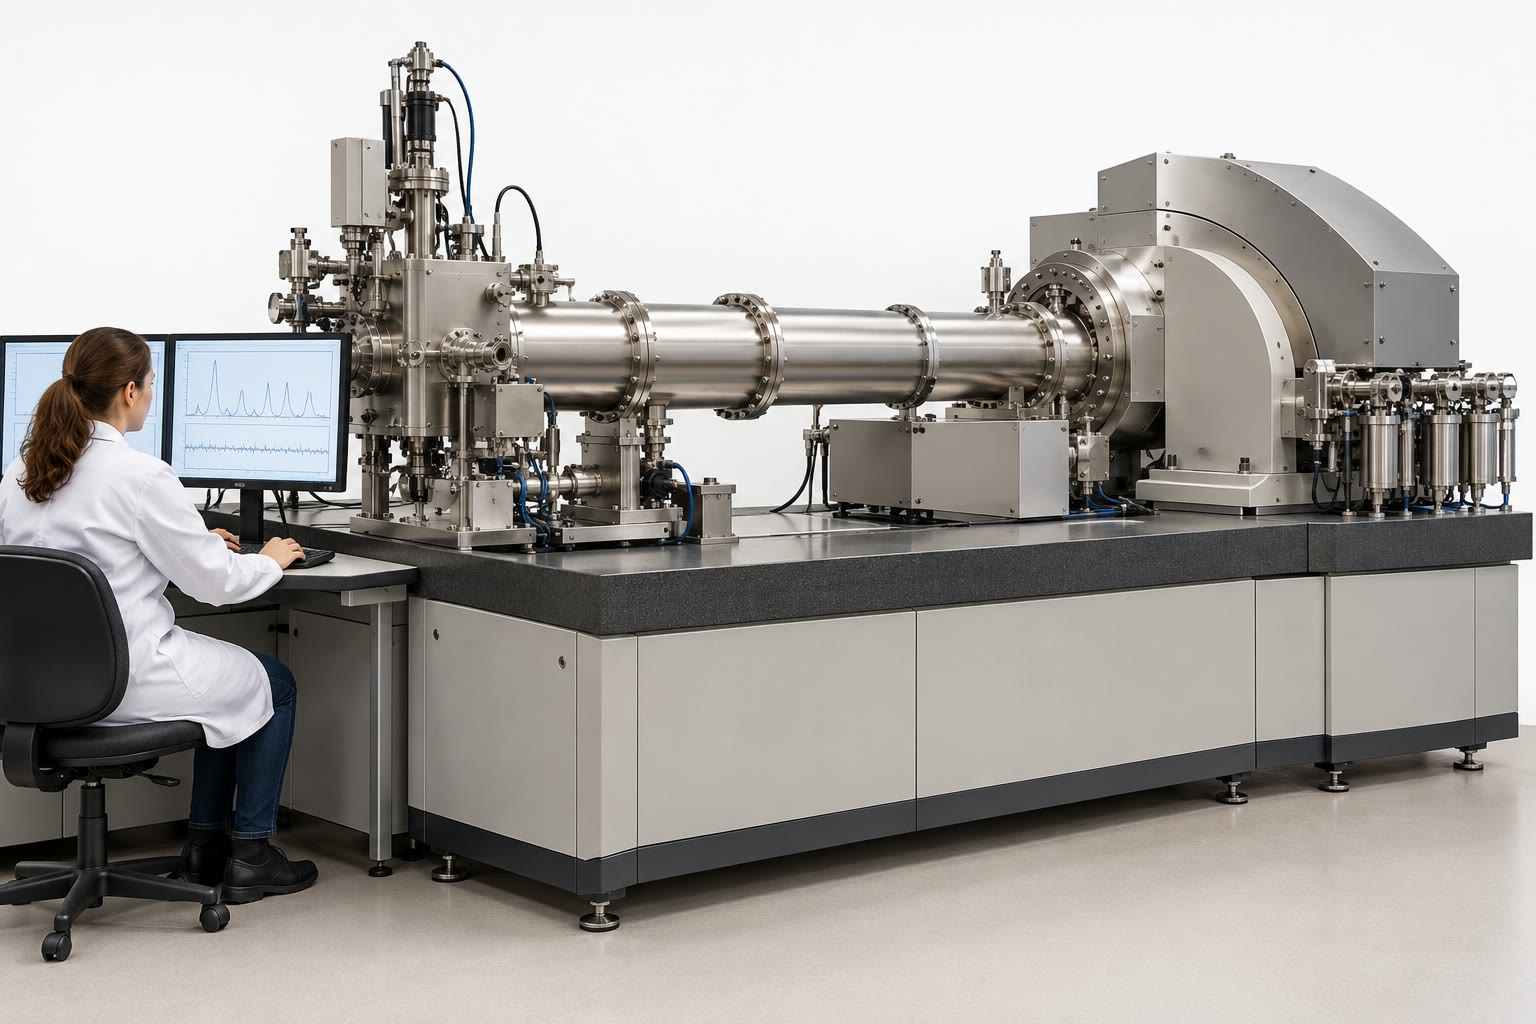
\includegraphics[width=\linewidth]{images/book4/ai/b2-isotope-lab.jpg}
\par\smallskip{\scriptsize किसी समस्थानिक प्रयोगशाला में एक बहु-संग्राहक द्रव्यमान
स्पेक्ट्रोमीटर (AI से बनाया गया चित्रण)।}
\end{minipage}
\end{inthelab}
% ledger: white:chur

\section{अभ्यास}

\begin{exercise}[$\star$]\label{exo:b2:isotope-geochemistry:1}
ट्रिस्टन दा कुन्हा के एक बेसाल्ट का $^{143}\mathrm{Nd}/^{144}\mathrm{Nd} = 0.51249$ है और
मंगाइया के एक का 0.51285। उनके और माध्य
MORB (0.513074) के $\varepsilon_{\mathrm{Nd}}$ परिकलित कीजिए। किन स्रोतों का Sm/Nd \omterm{def:b2:planet-formation-meteorites:chondrule}{कॉन्ड्राइटों} से ऊँचा रहा है?
\end{exercise}

\begin{exercise}[$\star$]\label{exo:b2:isotope-geochemistry:2}
अनुपात $^{18}\mathrm{O}/^{16}\mathrm{O}$ \omterm{def:b2:isotope-geochemistry:standards}{VSMOW} में \num{2.0052e-3} और
\omterm{def:b2:isotope-geochemistry:standards}{VPDB} में \num{2.0672e-3} है। \omterm{def:b2:isotope-geochemistry:standards}{VSMOW} पैमाने पर \omterm{def:b2:isotope-geochemistry:standards}{VPDB} का $\delta^{18}\mathrm{O}$
क्या है? एक कैल्साइट का $\delta^{18}\mathrm{O} = -2.0$ प्रति मिल (\omterm{def:b2:isotope-geochemistry:standards}{VPDB}) है; उसका अनुपात
और \omterm{def:b2:isotope-geochemistry:standards}{VSMOW} पैमाने पर उसका $\delta^{18}\mathrm{O}$ परिकलित कीजिए।
\end{exercise}

\begin{exercise}[$\star$]\label{exo:b2:isotope-geochemistry:3}
\qty{1.0}{Ga} पहले और \qty{4.567}{Ga} पहले CHUR का $^{143}\mathrm{Nd}/^{144}\mathrm{Nd}$
परिकलित कीजिए ($\lambda_{147} = \qty{6.524e-12}{\per\year}$,
$^{147}\mathrm{Sm}/^{144}\mathrm{Nd} = 0.1966$, आज 0.512638)।
\end{exercise}

\begin{exercise}[$\star$]\label{exo:b2:isotope-geochemistry:4}
किसी पर्वतीय स्टेशन के हिम-नमूने का $\delta^{18}\mathrm{O} = -18.0$ प्रति मिल है।
\omterm{prop:b2:isotope-geochemistry:mwl}{उल्कीय जल रेखा} कौन-सा $\delta\mathrm{D}$ पूर्वानुमानित करती है? एक झील के जल का
$\delta^{18}\mathrm{O} = -4.0$ और $\delta\mathrm{D} = -42$ प्रति मिल है: उसका ड्यूटेरियम
आधिक्य $d = \delta\mathrm{D} - 8\delta^{18}\mathrm{O}$ परिकलित कीजिए, और बताइए कि वह रेखा के ऊपर है या
नीचे।
\end{exercise}

\begin{exercise}[$\star\star$]\label{exo:b2:isotope-geochemistry:5}
रैखिक-वृद्धि प्रतिज्ञप्ति का $Q$ निकालिए। एक ग्रेनाइट में Sm \qty{6.0}{ppm}
और Nd \qty{30}{ppm} है (CI: 0.145 और \qty{0.457}{ppm})। उसका
$f_{\mathrm{Sm/Nd}}$, और \qty{500}{Myr} में उसके $\varepsilon_{\mathrm{Nd}}$ का परिवर्तन
परिकलित कीजिए।
\end{exercise}

\begin{exercise}[$\star\star$]\label{exo:b2:isotope-geochemistry:6}
एक भूपर्पटी \qty{2.7}{Ga} पहले
$\varepsilon_{\mathrm{Nd}} = +3.5$ वाले प्रावार से, $f_{\mathrm{Sm/Nd}} = -0.45$ के साथ, अलग हुई। रैखिक-वृद्धि प्रतिज्ञप्ति से
उसके आज के $\varepsilon_{\mathrm{Nd}}$ का अनुमान लगाइए। सटीक
परिकलन $-27.3$ देता है; सन्निकटन कितना भिन्न है, और वह बहुत
ऊँचा है या बहुत नीचा, और क्यों?
\end{exercise}

\begin{exercise}[$\star\star$]\label{exo:b2:isotope-geochemistry:7}
एक बेसाल्टी मैग्मा (Sr \qty{130}{ppm}, $^{87}\mathrm{Sr}/^{86}\mathrm{Sr} = 0.7030$)
एक ग्रेनाइट (Sr \qty{320}{ppm}, 0.7200) को आत्मसात करता है। 5, 10 और 20 प्रतिशत ग्रेनाइट वाले
मिश्रणों का $^{87}\mathrm{Sr}/^{86}\mathrm{Sr}$ परिकलित कीजिए।
दिखाइए कि $^{87}\mathrm{Sr}/^{86}\mathrm{Sr}$, $1/\mathrm{Sr}$ के सापेक्ष एक सरल रेखा है
और उसकी प्रवणता और अंतःखंड बताइए।
\end{exercise}

\begin{exercise}[$\star\star$]\label{exo:b2:isotope-geochemistry:8}
\qty{20}{\degreeCelsius} पर द्रव--वाष्प प्रभाजन गुणांकों 1.0098 ($^{18}$O) और 1.084 (D) के साथ,
महासागरीय जल (0, 0) के साथ साम्यावस्था वाली वाष्प के $\delta^{18}\mathrm{O}$ और $\delta\mathrm{D}$, और
जल से वाष्प तक की रेखा की प्रवणता $\delta\mathrm{D}/\delta^{18}\mathrm{O}$
परिकलित कीजिए।
\qty{0}{\degreeCelsius} (1.0117 और 1.111) पर दोहराइए। \omterm{prop:b2:isotope-geochemistry:mwl}{उल्कीय जल रेखा} से तुलना कीजिए।
\end{exercise}

\begin{exercise}[$\star\star$]\label{exo:b2:isotope-geochemistry:9}
महाद्वीपीय भूपर्पटी सिलिकेट पृथ्वी के द्रव्यमान का 0.51 प्रतिशत है और
औसतन \qty{27}{ppm} Nd रखती है, सिलिकेट पृथ्वी के \qty{1.25}{ppm} के सामने।
भूपर्पटी का $\varepsilon_{\mathrm{Nd}}$ $-15$ और सिलिकेट पृथ्वी का 0 लीजिए। नियोडिमियम का
कितना हिस्सा भूपर्पटी में है? यदि शेष प्रावार एकसमान होता, तो
उसका $\varepsilon_{\mathrm{Nd}}$ क्या होता? यदि शेष प्रावार कॉन्ड्राइटी है, तो $+8.5$ वाले
क्षीणित भंडार को नियोडिमियम का कितना हिस्सा धारण करना होगा?
\end{exercise}

\begin{exercise}[$\star\star\star$]\label{exo:b2:isotope-geochemistry:10}
दिखाइए कि रैखिक-वृद्धि प्रतिज्ञप्ति में उपेक्षित पदों का सापेक्ष
आकार लगभग $\lambda t/2$ है। पृथ्वी की आयु में यह कितना बड़ा है, और
यह $\varepsilon_{\mathrm{Nd}}$ में कितनी बड़ी त्रुटि उत्पन्न करता है,
$f = -0.45$ के लिए \qty{2.7}{Ga} में?
\end{exercise}

\begin{exercise}[$\star\star\star$]\label{exo:b2:isotope-geochemistry:11}
दो घटकों के Sr/Nd अनुपात 13.3 (A) और 5.0 (B) हैं। \omterm{prop:b2:isotope-geochemistry:mixing}{मिश्रण अतिपरवलय} की
उपपत्ति का प्रयोग करके, उस मिश्रण में A से आने वाले स्ट्रॉन्शियम का हिस्सा $s'$ ज्ञात कीजिए जिसमें A
नियोडिमियम का हिस्सा $s = 0.5$ देता है। $s$ के किस मान के लिए दोनों
हिस्से सबसे अधिक भिन्न होते हैं?
\end{exercise}

\begin{exercise}[$\star\star\star$]\label{exo:b2:isotope-geochemistry:12}
एक बॉक्स मॉडल के अनुसार \qty{4.5}{Ga} पहले पृथ्वी के बनने से महाद्वीपीय भूपर्पटी के वर्तमान आयतन,
\qty{7.2e9}{km^3}, का 2.3 से 2.6 गुना उत्पन्न हुआ, और 1.3 से 1.6
गुना नष्ट हुआ। जनन और विनाश की माध्य दरें
\unit{km^3} प्रति वर्ष में परिकलित कीजिए। उनकी तुलना क्षेपण क्षेत्रों की वर्तमान दरों,
प्रति वर्ष \qty{2.7}{km^3} जुड़ने और \qty{3.2}{km^3} हटने, से कीजिए।
\end{exercise}

\section{समस्या: तीन द्वीप, तीन प्रावार}

\begin{problem}[{सप्ताहांत समस्या --- तीन द्वीपों के लावाओं को
प्रावार सरणी पर रखना, मिश्रण को तीसरे घटक से अलग करना, और
पुनर्चक्रित अवसाद की आयु निकालना}]
\label{pb:b2:isotope-geochemistry:1}
एक काल्पनिक महासागर के तीन ज्वालामुखीय द्वीप, कोरा, वेल और आशा, नीचे दिए
समस्थानिक अनुपातों वाले बेसाल्ट उद्गारित करते हैं। एक भू-रसायनविद् उनके स्रोतों को दो
घटकों से मॉडल करती है: MORB के स्रोत जैसा एक \omterm{def:b2:isotope-geochemistry:reservoirs}{क्षीणित प्रावार} (Sr \qty{10}{ppm}, Nd
\qty{0.75}{ppm}, $^{87}\mathrm{Sr}/^{86}\mathrm{Sr} = 0.70282$,
$^{143}\mathrm{Nd}/^{144}\mathrm{Nd} = 0.51307$) और क्षेपण द्वारा प्रावार में लौटा एक पुराना
अवसाद (Sr \qty{200}{ppm}, Nd \qty{40}{ppm}, $0.72000$, $0.51141$;
$^{147}\mathrm{Sm}/^{144}\mathrm{Nd} = 0.110$, $^{87}\mathrm{Rb}/^{86}\mathrm{Sr} = 0.50$)।
कोरा: $0.70410$, $0.51278$; वेल: $0.70618$, $0.51242$; आशा: $0.70290$, $0.51288$
($^{87}\mathrm{Sr}/^{86}\mathrm{Sr}$, $^{143}\mathrm{Nd}/^{144}\mathrm{Nd}$)। आज CHUR:
$^{143}\mathrm{Nd}/^{144}\mathrm{Nd} = 0.512638$, $^{147}\mathrm{Sm}/^{144}\mathrm{Nd} =
0.1966$; $\lambda_{147} = \qty{6.524e-12}{\per\year}$, $\lambda_{87} =
\qty{1.3972e-11}{\per\year}$।

\medskip\noindent\textbf{भाग I --- द्वीपों को स्थान देना।}
\begin{enumerate}
\item दोनों घटकों का $\varepsilon_{\mathrm{Nd}}$ परिकलित कीजिए।
\item तीनों द्वीपों का $\varepsilon_{\mathrm{Nd}}$ परिकलित कीजिए।
\item पाँचों संघटनों को Sr--$\varepsilon_{\mathrm{Nd}}$ आरेख पर रखिए। कौन-से
द्वीप CHUR के समृद्ध पक्ष पर हैं?
\item आशा का स्ट्रॉन्शियम अनुपात लगभग \omterm{def:b2:isotope-geochemistry:reservoirs}{क्षीणित प्रावार} जैसा है पर
$\varepsilon_{\mathrm{Nd}}$ कहीं निम्न। प्रावार सरणी के सापेक्ष वह कहाँ आता है, और
अध्याय के किस द्वीप-समूह से मिलता-जुलता है?
\item लावाओं के समस्थानिक अनुपात उनके स्रोतों के अनुपात क्यों माने जा सकते हैं,
यद्यपि लावाओं के Sm/Nd और Rb/Sr उनके स्रोतों से बहुत भिन्न हैं?
\item $^{147}\mathrm{Sm}/^{144}\mathrm{Nd} = 0.12$ वाला कोरा का एक लावा \qty{1}{Myr} पुराना है।
उद्गार के बाद से उसका $^{143}\mathrm{Nd}/^{144}\mathrm{Nd}$ एप्सिलॉन इकाइयों में कितना
बढ़ा है? क्या इसका महत्त्व है?
\end{enumerate}

\noindent\textbf{भाग II --- दोनों घटकों का मिश्रण।}
\begin{enumerate}[resume]
\item उस मिश्रण की Nd सांद्रता और $^{143}\mathrm{Nd}/^{144}\mathrm{Nd}$ लिखिए
जिसमें अवसाद का द्रव्यमान-अंश $f$ है।
\item उन मिश्रणों का $\varepsilon_{\mathrm{Nd}}$ परिकलित कीजिए जिनमें $f = 0.5$, 1, 2 और 5
प्रतिशत है।
\item उन्हीं मिश्रणों का $^{87}\mathrm{Sr}/^{86}\mathrm{Sr}$ परिकलित कीजिए।
\item दिखाइए कि मिश्रणों का $^{87}\mathrm{Sr}/^{86}\mathrm{Sr}$, $1/\mathrm{Sr}$ के सापेक्ष एक सरल
रेखा है, और उसकी प्रवणता बताइए।
\item $K = (\mathrm{Sr}/\mathrm{Nd})_{\text{प्रावार}}/(\mathrm{Sr}/\mathrm{Nd})_{\text{अवसाद}}$ परिकलित कीजिए।
$f$ बढ़ने पर कौन-सा अनुपात, Sr या Nd, अवसाद की ओर तेज़ी से बढ़ता है?
\item अवसाद प्रावार की तुलना में Nd में कितने गुना, और Sr में कितने गुना समृद्ध है?
इन संख्याओं से समझाइए कि एक प्रतिशत अवसाद
$\varepsilon_{\mathrm{Nd}}$ को लगभग 11 इकाई क्यों खिसका देता है।
\item $f = 1$ प्रतिशत वाले मिश्रण के नियोडिमियम का कितना हिस्सा
अवसाद से आता है?
\end{enumerate}

\noindent\textbf{भाग III --- कितना अवसाद?}
\begin{enumerate}[resume]
\item Nd मिश्रण-समीकरण को $f$ के लिए हल कीजिए, मिश्रण का अनुपात $R$ दिया होने पर।
\item कोरा के लिए उसके नियोडिमियम से $f$ परिकलित कीजिए।
\item कोरा के लिए उसके स्ट्रॉन्शियम से $f$ परिकलित कीजिए। क्या दोनों मेल खाते हैं?
\item वेल के लिए उसके नियोडिमियम से और उसके स्ट्रॉन्शियम से $f$ परिकलित कीजिए।
\item आशा के लिए उसके नियोडिमियम से $f$ परिकलित कीजिए, और वह स्ट्रॉन्शियम अनुपात जो यह $f$
पूर्वानुमानित करता है। मापे गए मान से तुलना कीजिए: आशा के स्रोत के बारे में आप क्या
निष्कर्ष निकालते हैं?
\item अध्याय के आधार पर आशा के लिए एक तीसरा घटक सुझाइए, और वे
जनक--संतति अनुपात जो उसके रहे होंगे।
\end{enumerate}

\noindent\textbf{भाग IV --- अवसाद की आयु।}
\begin{enumerate}[resume]
\item अवसाद \qty{2.0}{Ga} पहले क्षेपित हुआ और तब से बंद है।
उस समय उसका $^{143}\mathrm{Nd}/^{144}\mathrm{Nd}$, CHUR का अनुपात और उसका
$\varepsilon_{\mathrm{Nd}}$ परिकलित कीजिए।
\item रैखिक-वृद्धि प्रतिज्ञप्ति से परिकलन फिर कीजिए।
\item \qty{2.0}{Ga} पहले अवसाद का $^{87}\mathrm{Sr}/^{86}\mathrm{Sr}$ परिकलित कीजिए।
\item \qty{2.0}{Ga} पहले, $\varepsilon_{\mathrm{Nd}}$ वाले चित्र की भूपर्पटी का
$\varepsilon_{\mathrm{Nd}} \approx -4.7$ था। क्या क्षेपण के समय अवसाद का मान
ऐसी युवा महाद्वीपीय भूपर्पटी के अपरदन से उत्पत्ति से संगत है?
\item सबसे अधिक समृद्ध द्वीप के स्रोत में पुनर्चक्रित अवसाद का द्रव्यमान-अंश बताइए,
जो इस समस्या की मुख्य संख्या है।
\end{enumerate}
\end{problem}
% ledger: white:chur, villa20:sm147, villa22:rb87, gale13:isotopes
